
In practice, writing the closed-form expression of the derivative of
a loss function $f$ w.r.t. the parameters of a deep neural network is hard
(and mostly unnecessary) as $f$ becomes complex. Instead, we define
computation graphs and use the automatic differentiation algorithms (typically backpropagation) to compute
gradients using the chain rule. For example, consider the expression

\begin{equation}
f(x, y) = (x+y)(y+1)
\end{equation}

Let's define intermediate variables $a$ and $b$ such that

\begin{equation}
a = x + y
\end{equation}
%
\begin{equation}
b = y + 1
\end{equation}
%
\begin{equation}
f = a \times b
\end{equation}
A computation graph for the ``forward pass'' through $f$ is shown in \figref{fig:graph}. 

\begin{figure}[h]
  \centering
    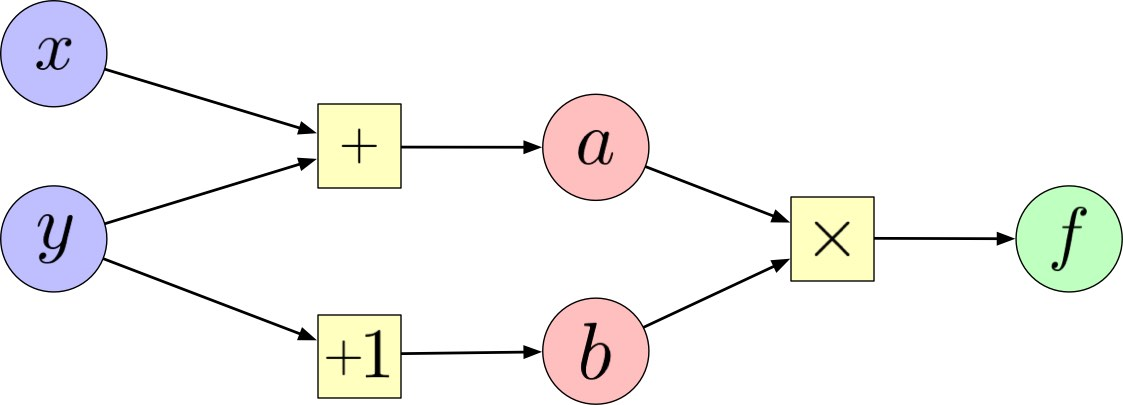
\includegraphics[width=0.5\textwidth]{assets/comp_graph_example.jpg}
    \caption{}
    \label{fig:graph}
\end{figure}

We can then work backwards and compute the derivative of $f$ w.r.t. each
intermediate variable ($\frac{\del f}{\del a}$, $\frac{\del f}{\del b}$) and
chain them together to get $\frac{\del f}{\del x}$ and $\frac{\del f}{\del y}$. \\

Let $\sigma(\cdot)$ denote the standard sigmoid function. Now, for the following vector function:

\begin{align}
f_1(w_1, w_2) &= \cos(w_1)\cos(w_2) + \sigma(w_2) \\
f_2(w_1, w_2) &= ln(w_1 + w_2) + w_1^2 w_2
\end{align}

\begin{enumerate}
\item Draw the computation graph. Compute the value of $f$ at $\vec{w} = (1, 2)$.
\item At this $\vec{w}$, compute the Jacobian $\frac{\del \vec{f}} {\del \vec{w}}$ using numerical differentiation (using $\Delta w$ = 0.01).
\item At this $\vec{w}$, compute the Jacobian using forward mode auto-differentiation.
\item At this $\vec{w}$, compute the Jacobian using backward mode auto-differentiation.
\item Don't you love that software exists to do this for us?
% making use of intermediate variables and reusing
%nodes (caching results) where necessary. Then apply the chain rule and compute
%$\frac{\del f}{\del w}$.
\end{enumerate}